\documentclass[a4paper, 11pt]{article}
\usepackage{comment} % enables the use of multi-line comments (\ifx \fi) 
\usepackage{lipsum} %This package just generates Lorem Ipsum filler text. 
\usepackage{fullpage} % changes the margin
\usepackage[a4paper, total={7in, 10in}]{geometry}
\usepackage[fleqn]{amsmath}
\usepackage{amssymb,amsthm}  % assumes amsmath package installed
\newtheorem{theorem}{Theorem}
\newtheorem{corollary}{Corollary}
\usepackage{graphicx}
\usepackage{tikz}
\usetikzlibrary{arrows}
\usepackage{verbatim}
\usepackage[numbered]{mcode}
\usepackage{float}
\usepackage{tikz}
    \usetikzlibrary{shapes,arrows}
    \usetikzlibrary{arrows,calc,positioning}

    \tikzset{
        block/.style = {draw, rectangle,
            minimum height=1cm,
            minimum width=1.5cm},
        input/.style = {coordinate,node distance=1cm},
        output/.style = {coordinate,node distance=4cm},
        arrow/.style={draw, -latex,node distance=2cm},
        pinstyle/.style = {pin edge={latex-, black,node distance=2cm}},
        sum/.style = {draw, circle, node distance=1cm},
    }
\usepackage{xcolor}
\usepackage{mdframed}
\usepackage[shortlabels]{enumitem}
\usepackage{indentfirst}
\usepackage{hyperref}
    
\renewcommand{\thesubsection}{\thesection.\alph{subsection}}

\newenvironment{problem}[2][Problem]
    { \begin{mdframed}[backgroundcolor=gray!20] \textbf{#1 #2} \\}
    {  \end{mdframed}}

% Define solution environment
\newenvironment{solution}
    {\textit{Solution:}}
    {}

\renewcommand{\qed}{\quad\qedsymbol}
%%%%%%%%%%%%%%%%%%%%%%%%%%%%%%%%%%%%%%%%%%%%%%%%%%%%%%%%%%%%%%%%%%%%%%%%%%%%%%%%%%%%%%%%%%%%%%%%%%%%%%%%%%%%%%%%%%%%%%%%%%%%%%%%%%%%%%%%
\begin{document}
%Header-Make sure you update this information!!!!
\noindent
%%%%%%%%%%%%%%%%%%%%%%%%%%%%%%%%%%%%%%%%%%%%%%%%%%%%%%%%%%%%%%%%%%%%%%%%%%%%%%%%%%%%%%%%%%%%%%%%%%%%%%%%%%%%%%%%%%%%%%%%%%%%%%%%%%%%%%%%
\large\textbf{Ben Smith} \hfill \textbf{Homework - \#1}   \\
Email: bxs566@case.edu \hfill ID: 3559750 \\
\normalsize Course: CSDS 337 - Compiler Design \hfill Term: Spring 2024\\
Instructor: Dr. Vipin Chaudhary \hfill Due Date: $5^{th}$ Feb, 2024 \\ \\
Number of hours delay for this Problem Set: \hfill 0\\
Cumulative number of hours delay so far: \hfill 0 \\ \\
I discussed this homework with: \hfill No one. \\
\noindent\rule{7in}{2.8pt}
%%%%%%%%%%%%%%%%%%%%%%%%%%%%%%%%%%%%%%%%%%%%%%%%%%%%%%%%%%%%%%%%%%%%%%%%%%%%%%%%%%%%%%%%%%%%%%%%%%%%%%%%%%%%%%%%%%%%%%%%%%%%%%%%%%%%%%%%
% Problem 1
%%%%%%%%%%%%%%%%%%%%%%%%%%%%%%%%%%%%%%%%%%%%%%%%%%%%%%%%%%%%%%%%%%%%%%%%%%%%%%%%%%%%%%%%%%%%%%%%%%%%%%%%%%%%%%%%%%%%%%%%%%%%%%%%%%%%%%%%
\begin{problem}{1}
What language is generated by the following grammars?
\begin{enumerate}[a]
    \item $S \longrightarrow 0 S 1 | 0 1 $
    \item $S \longrightarrow {\bf a} S {\bf b} S | {\bf b} S {\bf a} S | \epsilon $
    \item $S \longrightarrow  S + S | S * S | (S) | {\bf id}  $
\end{enumerate}

\end{problem}
\begin{solution}
    Your solutions go here
    \begin{enumerate}[a]
        \item All strings of length greater than or equal to four of an equal number of zeroes and ones, starting with all zeroes first and ending with the ones.
        \item All strings of an equal number of a's and b's.
        \item All mathematical expressions using id's with only addition, multiplication, and parentheses.
    \end{enumerate}
\end{solution}
\noindent\rule{7in}{2.8pt}

%%%%%%%%%%%%%%%%%%%%%%%%%%%%%%%%%%%%%%%%%%%%%%%%%%%%%%%%%%%%%%%%%%%%%%%%%
% Problem 2
%%%%%%%%%%%%%%%%%%%%%%%%%%%%%%%%%%%%%%%%%%%%%%%%%%%%%%%%%%%%%%%%%%%%%%%%%%%%%%%%%%%%%%%%%%%%%%%%%%%%%%%%%%%%%%%%%%%%%%%%%%%%%%%%%%%%%%%%

\begin{problem}{2}
Which of the following grammars are ambiguous? If ambiguous, show parse trees to substantiate.

\begin{enumerate}[a]
    \item $S \longrightarrow 0 S 1 | 0 1 $
    \item $S \longrightarrow {\bf a} S {\bf b} S | {\bf b} S {\bf a} S | \epsilon $
    \item $S \longrightarrow  S + S | S * S | (S) | {\bf id}  $
\end{enumerate}

\end{problem}
\begin{solution}
    Your solutions go here
    \begin{enumerate}[a]
        \item  $S \longrightarrow 0 S 1 | 0 1 $ is not ambiguous.

        \item $S \longrightarrow {\bf a} S {\bf b} S | {\bf b} S {\bf a} S | \epsilon $ is ambiguous.

              \begin{figure}[H]
                  \centering
                  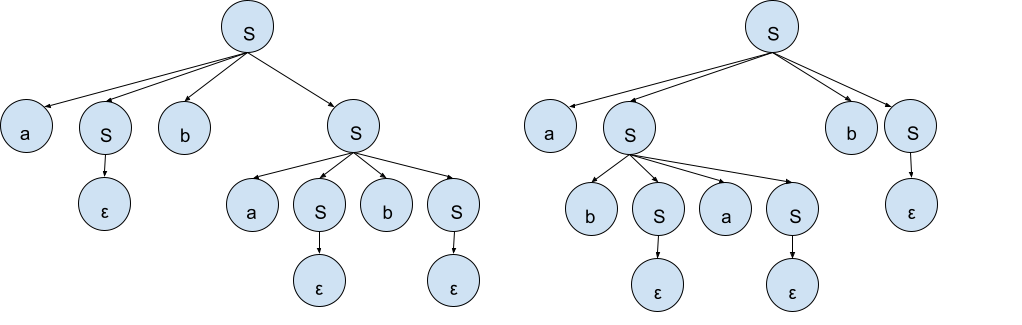
\includegraphics[scale=0.35]{337ps1q2b.png}
                  \caption{Two parse trees that generate the string "abab".}
                  \label{fig_2b}
              \end{figure}

        \item $S \longrightarrow  S + S | S * S | (S) | {\bf id}  $ is ambiguous.

              \begin{figure}[H]
                  \centering
                  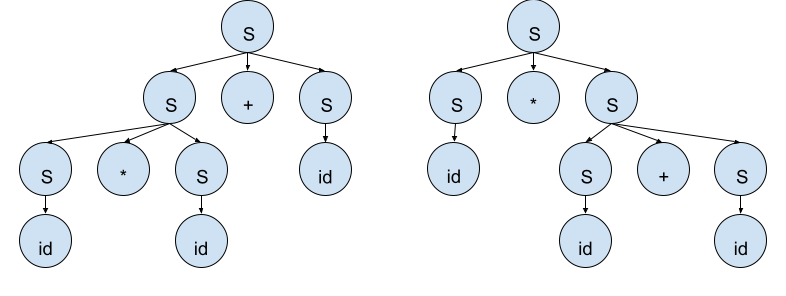
\includegraphics[scale=0.4]{337ps1q2c.png}
                  \caption{Two parse trees that generate the string "${\bf id} * {\bf id} + {\bf id}$".}
                  \label{fig_2c}
              \end{figure}

    \end{enumerate}
\end{solution}
\noindent\rule{7in}{2.8pt}

%%%%%%%%%%%%%%%%%%%%%%%%%%%%%%%%%%%%%%%%%%%%%%%%%%%%%%%%%%%%%%%%%%%%%%%%%
% Problem 3
%%%%%%%%%%%%%%%%%%%%%%%%%%%%%%%%%%%%%%%%%%%%%%%%%%%%%%%%%%%%%%%%%%%%%%%%%%%%%%%%%%%%%%%%%%%%%%%%%%%%%%%%%%%%%%%%%%%%%%%%%%%%%%%%%%%%%%%%

\begin{problem}{3}

\begin{enumerate}[a]
    \item For the predictive parser provided to you, execute the following program and submit the output.

          \begin{verbatim}
{
    int i; int j; float[10][10] a;
    i = 0;
    while ( i < 10 ) {
    	       j = 0;
            while ( j < 10 ) {
                a[i][j][j] = 0;
                j = j+1;
            }
            i = i+1;
    }
    i = 0;
    while ( i < 10 ) {
        a[i][i] = 1;
        i = i+1;
    }
}
\end{verbatim}

    \item For the predictive parser provided to you, execute the following program and submit the output.
          \begin{verbatim}
{
    int i; int j; float[20][20] a;
    i = 0;
    while ( i < 20 ) {
    	       j = 0;
            while ( j < 20 ) {
                a[i][j] = i + j;
                j = j+1;
            }
            i = i+1;
    }
    i = 0;
    while ( i < 20 ) {
        a[i][i] = 1;
        i = i+1;
    }
}
\end{verbatim}
\end{enumerate}
\end{problem}

\begin{solution}
    \begin{enumerate}[a]
        \item There was an error while parsing this code, which makes sense. At line 7, 3 array indices are used to get an element in a two-dimensional array. The output from the terminal is below:

              \lstinputlisting{3a.i}

        \item This example produced no errors and successfully generated intermediate code. There were no messages in the terminal. The output is below:

              \lstinputlisting{3b.i}
    \end{enumerate}
\end{solution}
%\lstinputlisting{SampleCode.m}
\noindent\rule{7in}{2.8pt}
%%%%%%%%%%%%%%%%%%%%%%%%%%%%%%%%%%%%%%%%%%%%%%%%%%%%%%%%%%%%%%%%%%%%%%%%%
\end{document}
